

\documentclass[]{article}
\usepackage[latin1]{inputenc}
\usepackage{ngerman}

\usepackage{graphicx}
\usepackage{geometry}

\geometry{verbose,a3paper, landscape, tmargin=20mm,bmargin=20mm,lmargin=25mm,rmargin=20mm}


\pagestyle{empty}

\begin{document}

\begin{figure}

\includegraphics[scale=0.15]{symgraph.pdf}
\caption{Symbolische L�sung}
\end{figure}

\begin{figure}
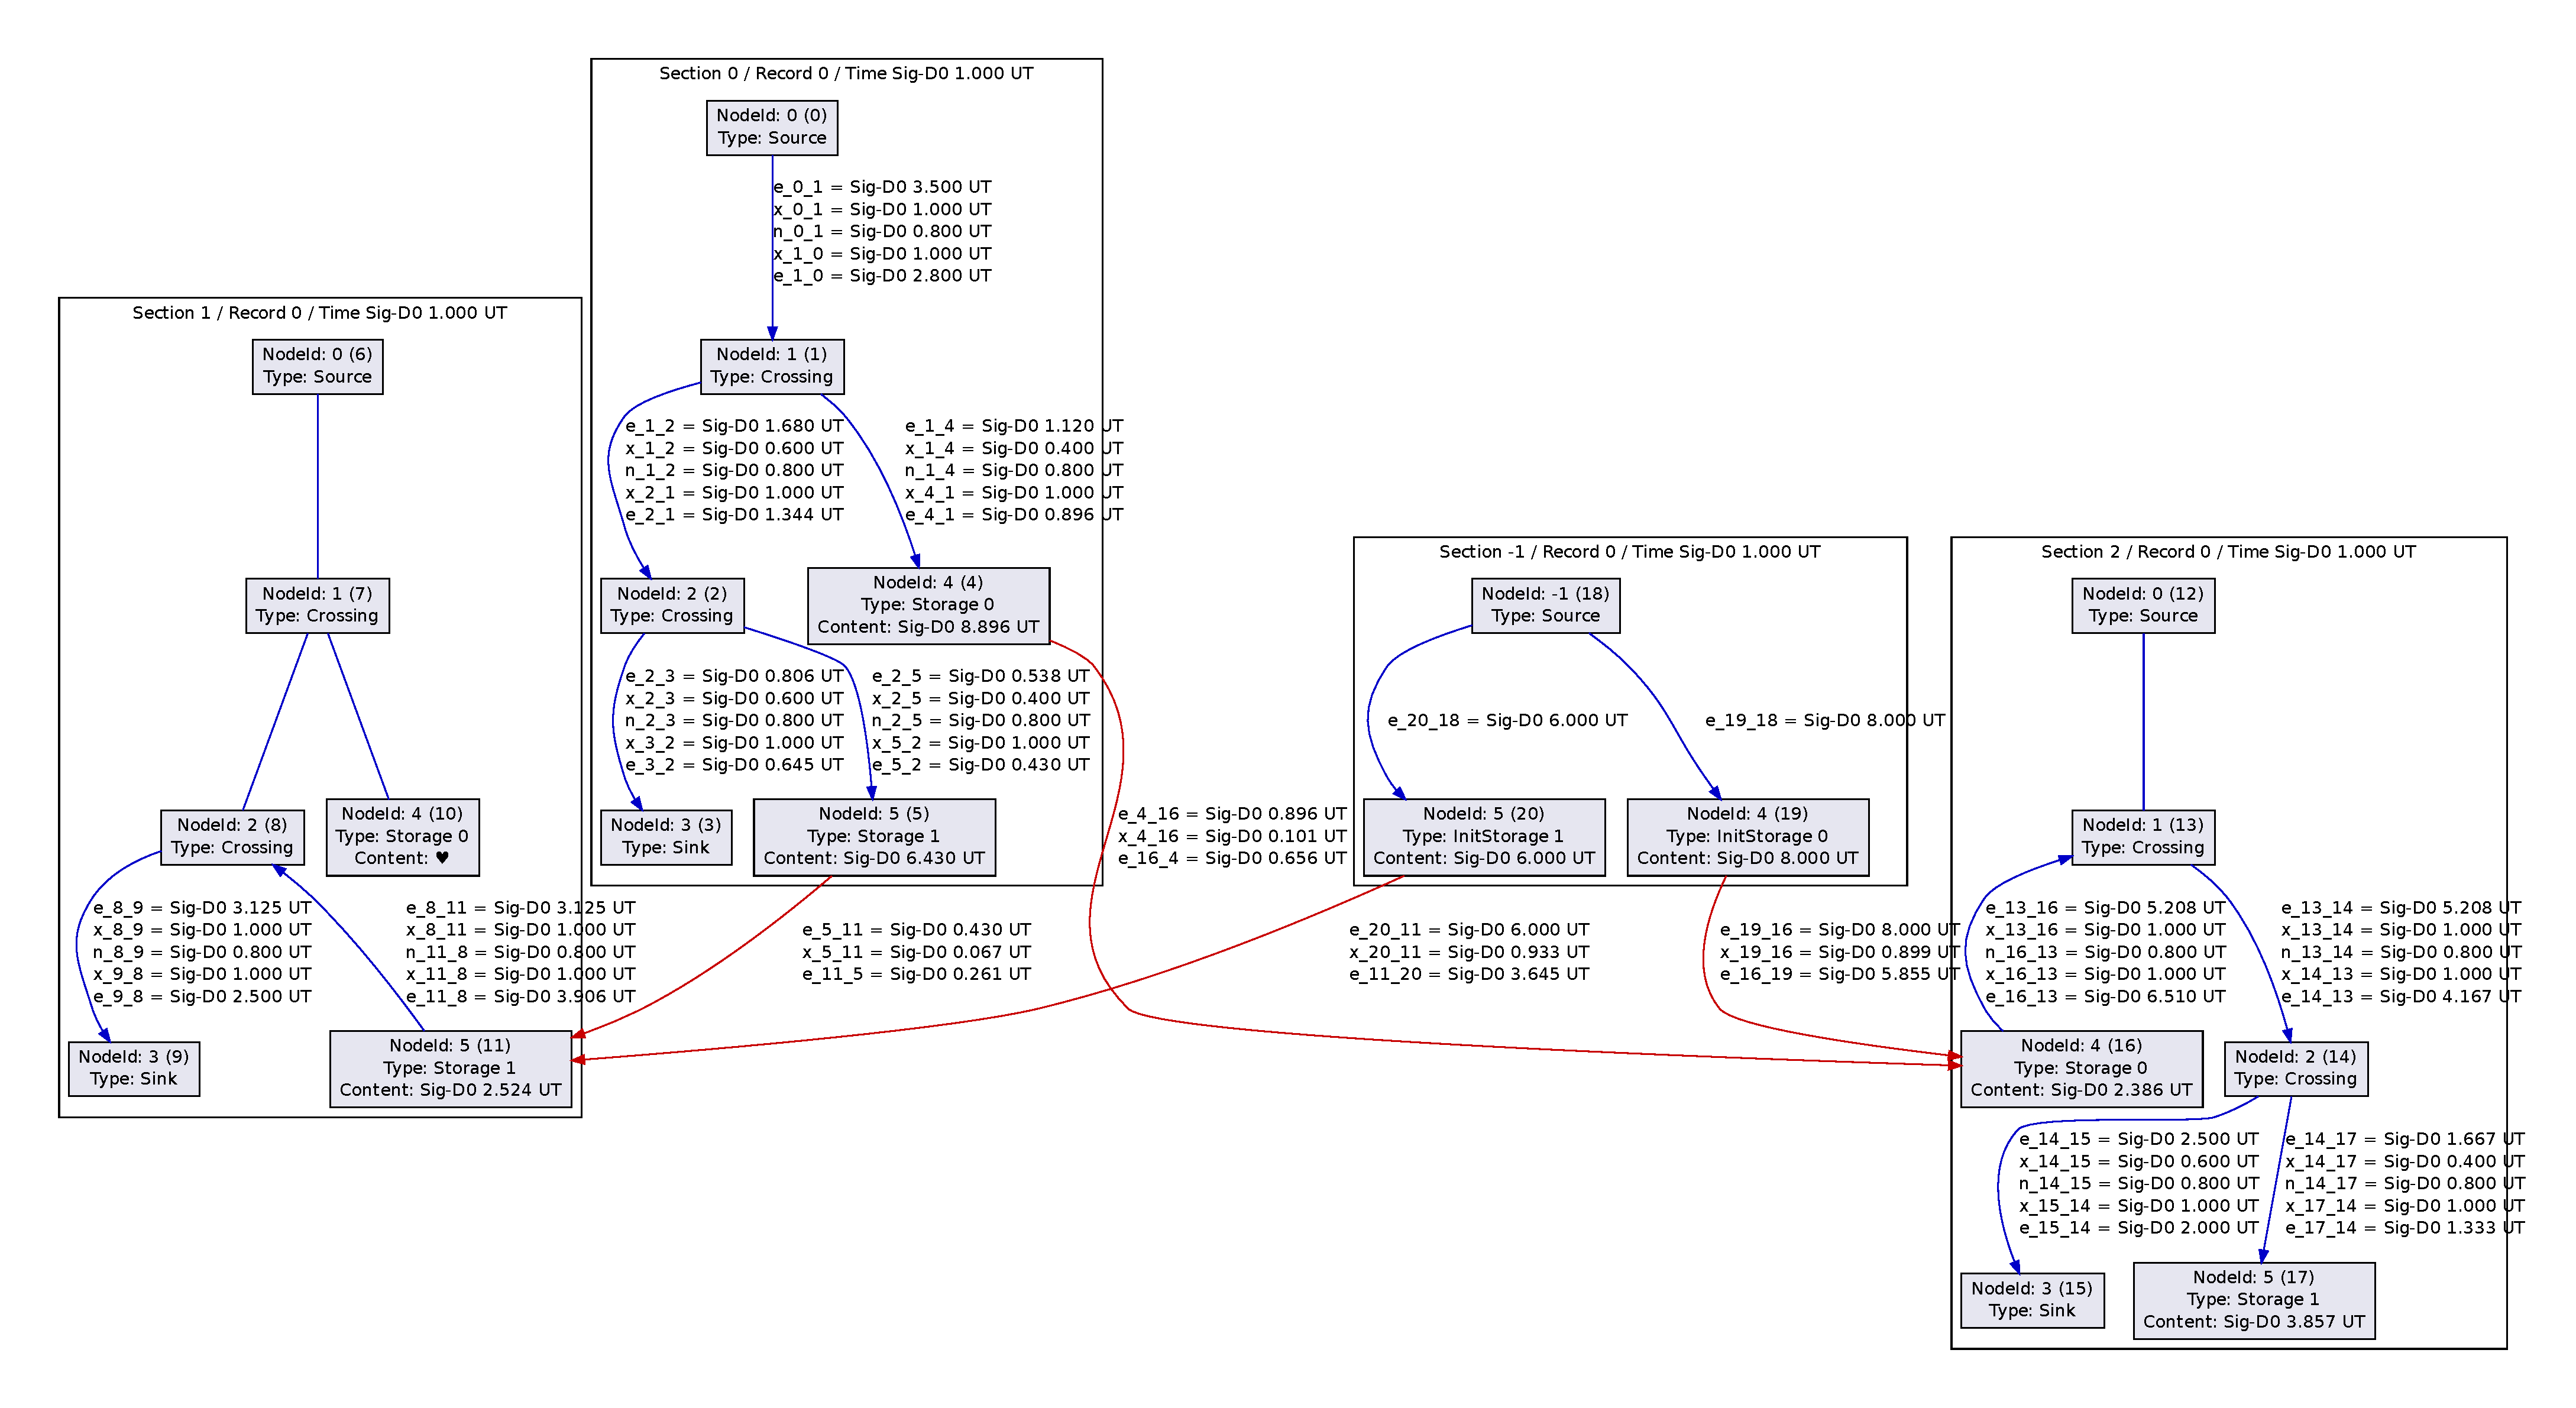
\includegraphics[scale=0.43]{numgraph.pdf}
\caption{Numerisch L�sung. Gegeben wurden $\Delta t_{i.j} = 1.0$, $P_{-1.0\_19.18} = 8.0$, $P_{-1.0\_20.18} = 6.0$, $P_{0.0\_0.1} = 3.5$, $P_{2.0\_15.14} = 2.0$, $P_{1.0\_9.8} = 2.5$, $\eta_{i.j\_k.l} = 0.8$, $x_{0.0\_1.2} = x_{0.0\_2.3} = x_{2.0\_14.15} = 0.6$, $x_{0.0\_1.4} = x_{0.0\_2.5} = x_{2.0\_14.17}  = 0.4$}
\end{figure}

\end{document}
